\let\negmedspace\undefined
\let\negthickspace\undefined
\documentclass[journal]{IEEEtran}
\usepackage[a5paper, margin=10mm, onecolumn]{geometry}
%\usepackage{lmodern} % Ensure lmodern is loaded for pdflatex
\usepackage{tfrupee} % Include tfrupee package
\setlength{\headheight}{1cm} % Set the height of the header box
\setlength{\headsep}{0mm}     % Set the distance between the header box and the top of the text
\usepackage{gvv-book}
\usepackage{gvv}
\usepackage{cite}
\usepackage{amsmath,amssymb,amsfonts,amsthm}
\usepackage{algorithmic}
\usepackage{graphicx}
\usepackage{textcomp}
\usepackage{xcolor}
\usepackage{txfonts}
\usepackage{listings}
\usepackage{enumitem}
\usepackage{mathtools}
\usepackage{gensymb}
\usepackage{comment}
\usepackage[breaklinks=true]{hyperref}
\usepackage{tkz-euclide} 
\usepackage{listings}
% \usepackage{gvv}                                        
\def\inputGnumericTable{}                                 
\usepackage[latin1]{inputenc}                                
\usepackage{color}                                            
\usepackage{array}                                            
\usepackage{longtable}                                       
\usepackage{calc}                                             
\usepackage{multirow}                                         
\usepackage{hhline}                                           
\usepackage{ifthen}                                           
\usepackage{lscape}
\begin{document}

\bibliographystyle{IEEEtran}
\vspace{3cm}
\parindent 0px

\title{9.4.21}
\author{EE24BTECH11050 - Pothuri Rahul}
% \maketitle
% \newpage
% \bigskip
{\let\newpage\relax\maketitle}

\renewcommand{\thefigure}{\theenumi}
\renewcommand{\thetable}{\theenumi}
\setlength{\intextsep}{10pt} % Space between text and floats


\numberwithin{equation}{enumi}
\numberwithin{figure}{enumi}
\renewcommand{\thetable}{\theenumi}

\textbf{Question:} \\
In a bank,principal increases continuously at the rate of $5\%$ per year. An amount of rupees $1000$ is deposited with this bank. How much will it worth after 10 years $\brak{e^{0.5} = 1.648}$ \\ \\
\solution 
\begin{table}[h!]
    \centering
    \begin{tabular}[12pt]{|c|c|}
     \hline
     {variable} & {description}\\
     \hline
     $P$ & Principle at any time t\\
     \hline
     $t$ & time in years\\
     \hline
     $C$ & primary arbitrary constant\\
     \hline
     $C_1$ & secondary arbitrary constant\\
     \hline
     $P_0$ & initial principle amount\\
     \hline
     
\end{tabular}

    \caption{Variables Used}
    
\end{table}
\\
\solution Let P be the principle at any time t. According to the given problem, Rate of change in principle can be given as 
\begin{align}
\frac{dP}{dt} = \brak{\frac{5}{100}} \times P \label{1}
\end{align}
\begin{align}
\frac{dP}{dt} = \brak{\frac{P}{20}} \label{2}
\end{align}
Seperating the variables in the equation \eqref{2}, We get 
\begin{align}
\frac{dP}{P}=\frac{dt}{20} \label{3}
\end{align}
On integrating both sides
\begin{align}
\int \frac{dP}{P}=\int \frac{dt}{20} \label{4} \\
log P = \frac{t}{20}+C \label{5} \\
P=e^{\frac{t}{20}+C} \label{6} \\
P=e^{\frac{t}{20}} . e^{C} \label{7} \\
P=e^{\frac{t}{20}} . C_1 \label{8}
\end{align}
Given, at time t=0,$P_0$=1000 then, from \eqref{8}
\begin{align}
1000=C_1 \label{9}
\end{align}
Principle can be given as 
\begin{align}
P = 1000 \times e^{\frac{t}{20}} \label{10}
\end{align}
At time t=10,Principle can be given as \\
\begin{align}
P =1000 \times e^{\frac{10}{20}} \\
P =1000 \times e^{0.5} \\
P = 1000 \times 1.648 \\
P = 1648
\end{align}
\begin{figure}[htbp] % Positioning options: here, top, bottom, page
    \centering
    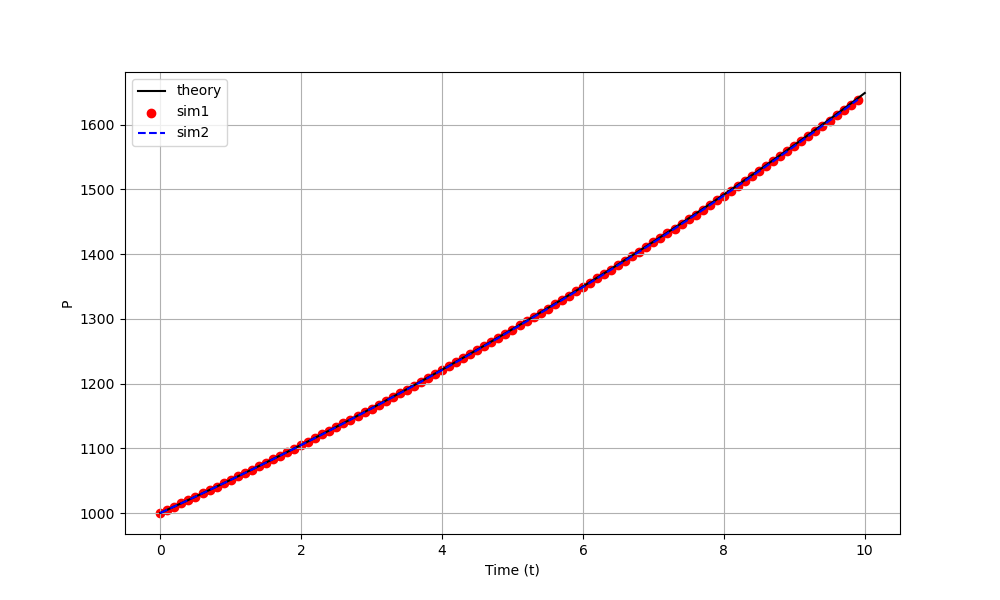
\includegraphics[width=\textwidth]{fig/plot.png} % Replace "filename" with your image file
    \caption{Plot}
\end{figure}



\end{document}
